
\section{问题背景}

在乡村振兴与农业现代化背景下,科学规划并高效利用有限土地,对保障区域粮食安全和促进乡村经济可持续发展至关重要。该问题涉及资源配置的运筹学建模,同时关联生态经济中的经济—生态系统相互作用和区域经济的内生增长机制。作物生产与品种选择受地域、气候和土壤等自然条件约束;其经济效益则依赖于市场需求、生产成本与销售价格等动态变量。基于此,需要制定兼顾经济产出最大化、生态稳定性与风险应对能力的长期种植策略。

本研究以华北某山区乡村为对象。该乡村兼具露天耕地与设施大棚等多类型土地资源,并受轮作制度、豆类种植比例及田间管理可及性等多重约束。上述现实因素构成了一个多维约束的决策环境。为此,本文采用系统的数学建模方法,构建覆盖2024至2030年的最优种植方案,以期为土地高效利用与经济稳健增长提供数据驱动的决策支持。


\section{问题重述}

问题一:在所有经济与生产参数取基准值且保持不变的条件下,针对 2024–2030 年规划期,求解最优种植结构以最大化七年累计利润。分别在两种需求情景下求解:(i)产量超出预期的部分无法销售;(ii)超出部分以基准价格的 50\% 出售。

问题二:在问题一框架上引入参数不确定性。考虑预期销售量、单位面积产量、单位面积种植成本和销售价格在给定区间内的波动,设计一个在整个规划期内保持不变的单一种植方案,以收益—风险权衡为目标,提升方案鲁棒性,并在不利市场与生产情景下保持经济绩效稳定。

问题三:在问题二基础上纳入作物间的替代性与互补性,以及预期销售量、销售价格与种植成本的相关结构。基于这些关系的建模与放好着呢,求解可随市场参数变化更新的自适应种植策略,并与问题二的鲁棒方案进行对比评估。


\section{问题分析}

对于问题一,其在确定性前提下提出:研究对象为多周期、多地块、多品类的资源分配问题,且假定所有生产与市场参数为已知且恒定,目标为在规划期内实现累计利润最大化。该设定与古典微观经济学中厂商理论的理性与利润最大化假设一致,因此在既定资源与农艺约束下的最优决策过程可被视为对单一目标决策主体的数学建模。由此,该问题可形式化为一个混合整数线性规划(MILP)模型,以便在约束条件下求解最优种植策略。

对于问题二,其本质上是将确定性优化推广到不确定情形:预期销量、单位产量、单位种植成本与销售价格作为在预设区间内波动的有界不确定量,且题设未给出其概率分布。因缺乏分布信息,基于概率分布的随机规划方法不可行,因此应采用仅依赖波动边界的建模策略,即鲁棒优化。鲁棒优化通过最大化最坏情形下的性能以体现风险规避倾向,相较于以期望收益为目标的方法更侧重最低收益保障与下行风险控制,从而在数据有限的条件下生成更为审慎且性能稳定的种植方案。

对于问题三,其在模型中引入作物间的替代性与互补性以及价格—需求反馈等系统性相互作用。由于这些相互作用产生显著的动态非线性,模型目标函数无法用封闭的解析表达式精确表示,故基于显式解析模型的优化方法(包括鲁棒优化)难以适用。因而应将该问题视为黑箱优化问题,并采用仿真—优化框架:首先构建能够再现关键市场与生产动态的高保真仿真器;其次采用不依赖问题解析形式的全局搜索算法在方案空间中寻优;最后通过仿真对所得自适应种植策略的性能与稳健性进行评估,并与问题二的鲁棒方案比较。

我们最终的框架如图\ref{fig:all}

\begin{figure}[htbp]
	\centering
	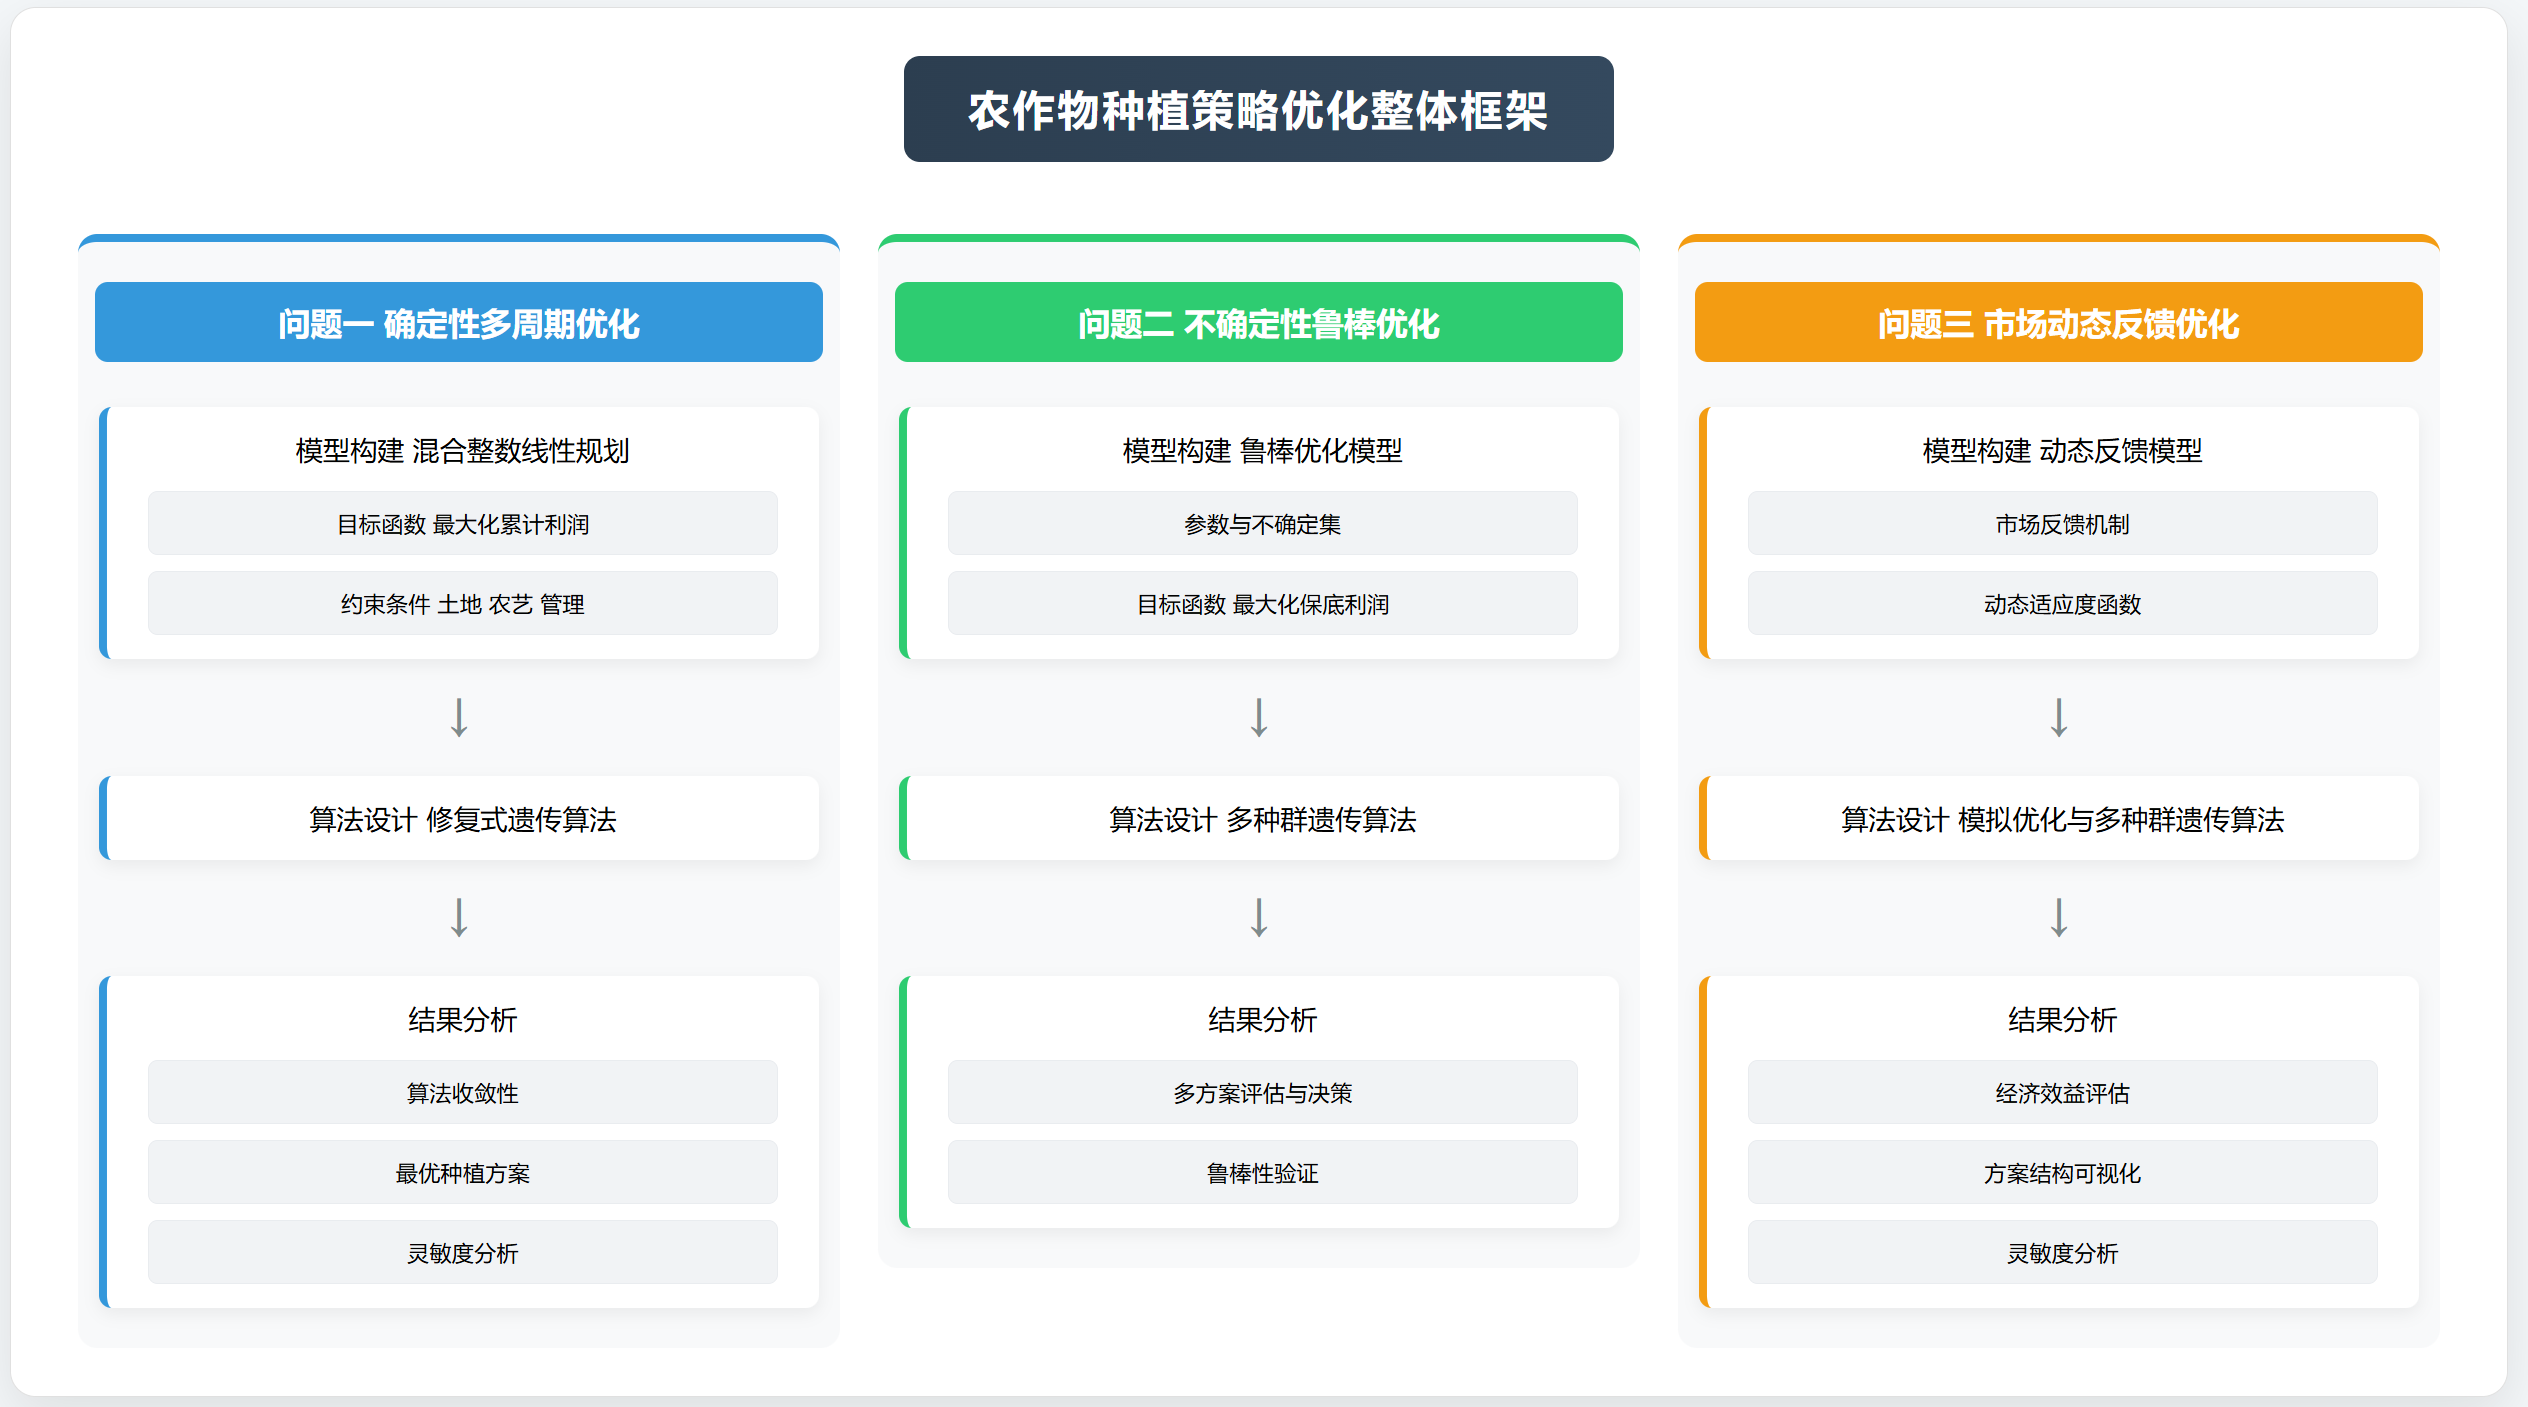
\includegraphics[width=\textwidth]{figs/1前置/全文框架.png}
	\caption{整体框架}
	\label{fig:all}
\end{figure}


\section{模型假设}


为确保数学模型的有效性与针对性,并明确其适用边界,我们提出以下四条基本假设:

\begin{enumerate}
    \item 模型所使用的全部历史数据均视为准确可靠。2023年的产销数据被视为代表了市场的均衡状态。

    \item 该乡村在农产品市场中被视为价格接受者。其自身的任何生产决策所导致的供给量变化,均不足以对该作物的市场结算价格产生实质性影响。

    \item 模型的经济效益评估聚焦于种植环节。所有计划销售的农产品,无论是正常价格或降价销售,均假定在当季完成交易。模型不包含仓储、物流、交易损耗等生产后环节的成本与收益。

    \item 在规划期内,所有种植活动所需的人力、设备、技术及其他生产资料均能得到充分供应,不构成生产决策的限制因素。

\end{enumerate}


\section{符号说明}

\begin{table}[H]
	\centering
	\caption{符号说明}
	\begin{tabular}{ll}
		\toprule
		符号                 & 说明                                \\
		\midrule

		$i, I$             & 地块的索引与集合                          \\
		$j, J$             & 作物的索引与集合                          \\
		$k, K$             & 季节的索引与集合                          \\
		$y, Y$             & 年份的索引与集合(2024-2030)               \\
		$J_{\text{bean}}$  & 所有豆类作物的集合                         \\

		$A_i$              & 地块$i$ 的可用面积                       \\
		$C_j$              & 作物$j$ 的单位面积种植成本                   \\
		$P_j$              & 作物$j$ 的单位重量销售价格                   \\
		$\text{Yield}_j$   & 作物$j$ 的单位面积产量                     \\
		$\text{Demand}_j$  & 作物$j$ 的每季预期市场销售量                  \\
		$\text{Past}_{ij}$ & 地块$i$ 在2023年是否种植了作物 $j$ 的0-1参数    \\
		$S_{ijk}$          & 地块$i$ 在季节 $k$ 是否适宜种植作物 $j$ 的0-1参数 \\
		$A_{\min}$         & 单个地块上允许种植某种作物的最小面积阈值              \\
		$N_j$              & 作物$j$ 在单季内允许种植的最大分散地块数量           \\
		$M$                & 大M方法中的一个足够大的正数                    \\
		\bottomrule
	\end{tabular}
\end{table}